\chapter{Crittografia a chiave pubblica} \label{ch:publickey}
\section{Introduzione}
La crittografia a chiave pubblica (\textbf{public key cryptogarphy}) (talvolta detta anche crittografia asimmetrica (\textbf{asymmetric cryptography}) fu pubblicamente introdotta nel 1975, anche se alcune voci sostengono che l'NSA già la utilizzasse da diverso tempo. Diversamente dalla crittografia a chiave segreta non prevede la \textbf{condivisione di un segreto}. Ogni entità ha due chiavi:
\begin{itemize}
	\item una chiave privata da \textbf{non rivelare} a nessuno
	\item una chiave pubblica da rivelare preferibilmente a tutto il mondo
\end{itemize}

\subsubsection{Terminologia e notazione}
Per convenzione non si userà il termine \textbf{chiave segreta} in luogo di \textbf{chiave privata}, per distinguere il concetto di chiave segreta utilizzata nel contesto di un algoritmo a crittografia simmetrica e chiave privata nel contesto di un algoritmo di crittografia asimmetrica. In base all’aggettivo della chiave sarà quindi immediato risalire allo schema di crittografia usato.
\begin{figure}[htbp]
	\centering%
	\subfigure%
	{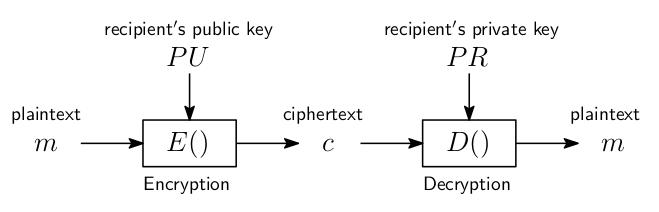
\includegraphics[height=13cm, width=10cm, keepaspectratio]{Immagini/chiave_pubblica/chiave_pubblica_schema.png}}
	\caption{Schema a blocchi crittografia a chiave pubblica \label{fig:pubblica_schema_blocchi}} 	
\end{figure}
Per quanto riguarda la notazione faremo riferimento alla \figurename~\ref{fig:pubblica_schema_blocchi}, in cui:
\begin{itemize}
	\item \textbf{PU} rappresenta la chiave \textbf{Pubblica}; ad esempio $PU_B$ indica la chiave pubblica di Bob
	\item \textbf{PR} rappresenta la chiave \textbf{Privata}; ad esempio $PR B$ indica la chiave privata di Bob
\end{itemize}
Cifratura e decifratura sono due funzioni matematiche che sono l'una l'inverso dell’altra:
\begin{equation}
m = D(PR, c) = D(PR, E (PU, m))
\end{equation}

\subsubsection{Firma digitale}
La tecnologia a chiave pubblica consente anche di generare una \textbf{firma digitale} su un messaggio (ovvero garantirne l'autenticità). Basta infatti invertire il ruolo delle chiavi, come mostrato in \figurename~\ref{fig:pubblica_schema_firma}. In questo contesto le funzioni E() e D() vengono denominate S()(Sign) e V()(Verify). 
\begin{figure}[htbp]
	\centering%
	\subfigure%
	{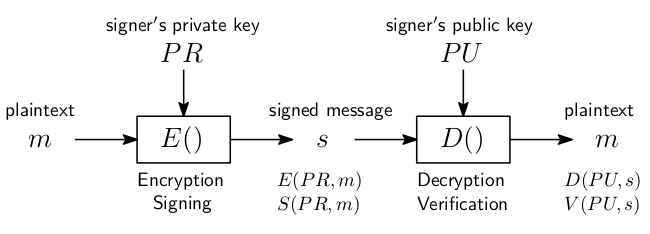
\includegraphics[height=13cm, width=10cm, keepaspectratio]{Immagini/chiave_pubblica/chiave_pubblica_firma.png}}
	\caption{Schema a blocchi crittografia a chiave pubblica \label{fig:pubblica_schema_firma}} 	
\end{figure}

La crittografia a chiave pubblica si basa su alcuni risultati nell'ambito della teoria dei numeri. Si esamineranno i seguenti schemi di cifratura a chiave pubblica: 
\begin{itemize}
\item RSA usata per cifrare e per calcolare la firma digitale
\item ElGamal e DSS, usati per la firma digitale
\item Diffie-Hellman, permette di stabilire un segreto condiviso, ma non fornisce alcun algoritmo che usa effettivamente tale segreto
\end{itemize}
L'unico aspetto comune a tutti gli algoritmi di crittografia a chiave pubblica è la presenza di due quantità correlate: una chiave segreta e una chiave pubblica.
\section{Aritmetica modulare}
La maggior parte degli algoritmi a chiave pubblica si basano sull'aritmetica modulare: fissato un intero $ n>1 $, l'aritmetica modulare considera l'insieme degli interi non negativi minori di
$n: $\{$0, 1, 2,..., n-1$\}, effettua operazioni ordinarie come l'addizione e la moltiplicazione, e sostituisce il risultato $x$ con il resto $r$ della divisione intera di $x$ per $n$. Il risultato finale viene detto modulo n o $mod \, n$. \\
Definiamo l'inverso moltiplicativo di $k$, indicato con $k^{-1}$, come quel numero che moltiplicato per $k$ dà 1, cioè $kk^{-1} \, mod \, n = 1 \, mod \, n$. Fissato n, non tutti i numeri hanno un inverso moltiplicativo $mod \, n$. Si osservi inoltre che, se $k$ ammette un inverso moltiplicativo $mod \, n $, esiste un unico inverso moltiplicativo $k^{-1} < n$. La moltiplicazione $mod \, n$ di per sé non costituisce un cifrario sicuro,ma funziona, nel senso che la moltiplicazione per $k$ produce un mescolamento dell'input; la decifratura può ottenersi moltiplicando per $k^{-1}$.\\ Trovare un inverso moltiplicativo $k^{-1}$ nella aritmetica $mod \, n$, non è affatto banale se $n$ è molto grande. Esiste un modo efficiente per risolvere tale problema, noto come algoritmo di Euclide: \begin{itemize}
\item dati $x$ ed $n$, con $x<n$, l'algoritmo di Euclide trova il
numero $y<n$ tale che $xy \, mod \, n = 1$, ammesso che un siffatto $y$ esista.\end{itemize} 
Quali sono dunque gli inversi moltiplicativi $mod \, n$? E' sufficiente trovare i numeri \textit{relativamente primi} con $n$, cioè tali che se $x$ è uno di questi numeri, si ha che $MCD(x,n) = 1$. Se $n$ è un numero primo, tutti gli interi positivi $x<n$ ammettono un inverso moltiplicativo $mod \, n$, che indichiamo con $x^{-1}$.\\ \\
\textbf{Funzione di Eulero o totiente:} \{$i \in Z, 0 < i < n: MCD(i,n) = 1$\} \\

Se $n$ è primo, tutti gli interi da 1 a $n-1$ sono relativamente primi con $n$, per cui $\phi(x) = n - 1$. Se $n = pq$, dove p e q sono numeri primi maggiori di 1, allora $\phi(n) = (p-1)(q-1)$. \\
Sia adesso $n > 1$ un intero privo di quadrati(cioè dove non compaiono fattori al quadrato nella sua scomposizione in fattori primi), detto anche square free, allora per ogni $y > 0$, si ha: \begin{center}
$x^y \, mod \, n = x^{(y + \phi(n) )} \, mod \, n$
\end{center} Ne segue che, se $ y = 1 \, mod \, \phi(n) $, ovvero se $y = 1 + k \phi(n) $, con $k \in Z$, si ha $x^y \, mod \, n = x \, mod \, n $. Tale risultato è sfruttato dall'algoritmo RSA.

\section{RSA}

RSA è un algoritmo di cifratura(a blocchi) a chiave pubblica, la cui lunghezza è variabile(solitamente si considerano chiavi di lunghezza pari ad almeno 512 bit). Anche la lunghezza dei blocchi è variabile: un blocco di testo in chiaro deve avere lunghezza minore di quella della chiave, mentre un blocco di testo cifrato è lungo come la chiave. \\
RSA è computazionalmente molto più lento degli algoritmi a chiave segreta più popolari come DES, IDEA e AES, per cui difficilmente viene usato per cifrare messaggi lunghi. Generalmente viene usato per cifrare una chiave segreta $K$, utilizzata per cifrare un messaggio usando un algoritmo a chiave segreta. RSA può essere usato dunque sia per cifrare/decifrare messaggi sia per la firma digitale di messaggi. In entrambi i casi bisogna disporre della coppia $<chiave \, pubblica, \,  chiave \, privata>(<PU,PR>)$. \\
I passi da seguire per generare la chiave pubblica e la chiave privata sono: \begin{enumerate}
\item Scegliere due numeri primi $p$ e $q$ molto grandi(circa 256 bit ciascuno) tali che $n = pq$. E' fondamentale che $p$ e $q$ rimangano segreti, cosicchè fattorizzare $n$ sia computazionalmente impraticabile. 
\item Scegliere un numero $e$ che sia relativamente primo rispetto a $\phi(n) = (p-1)(q-1)$.
\item Calcolare l'inverso moltiplicativo $d$ di $e \, mod \, \phi(n)$, cioè tale che sia $(d \cdot e ) \, mod \, \phi(n) \, = 1$.
\item La chiave pubblica è $PU = <e,n>$, mentre la chiave privata è $PR = <d,n>$.
\end{enumerate}
Per quanto riguarda la \textbf{cifratura}/\textbf{decifratura}, siano $PU$ e $PR$ la chiave pubblica e la chiave privata del destinatario, $m$ il messaggio da cifrare. La procedura da seguire è la seguente: \begin{itemize}
\item il mittente, utilizzando la chiave pubblica $PU$ del destinatario, cifra il messaggio ottenendo $c = m^e \, mod \, n$
\item il destinatario, usando la propria chiave privata $PR$, decifra $c$ calcolando $m = c^d \, mod \, n$. \end{itemize}
\textbf{Dimostrazione.} Poste le seguenti proprietà: \begin{itemize}
\item se $m<n$, $ \, m \, mod \, n\,=\,n$
\item $(x^a \, mod \, n)^b \, mod \, n \, = \, x^{ab} \, mod \, n$
\item $(e \cdot d) \, mod \, \phi(n) = 1$
\end{itemize}
Se $c=E(PU,m) = m^e \, mod \, n \, \Rightarrow m=D(PR,c) = c^d \, mod \, n = (m^e \, mod \, n)^d \, mod \, n = m^{ed} \, mod \, n = m^{1 \, mod \, \phi(n)} \, mod \, n = m \, mod \, n = m$. \\ \\
Per la \textbf{firma digitale} invece sia $PR$ la chiave privata del firmatario del messaggio e sia $PU$ la sua chiave pubblica: \begin{itemize}
\item il firmatario, usando la propria chiave privata $PR$, calcola la firma digitale $s = m^d \, mod \, n$;
\item chiunque desideri verificare l'autenticità della firma, può farlo usando la chiave pubblica $PU$ del firmatario e calcolando $m = s^e \, mod \, n$.
\end{itemize}
La dimostrazione è per la firma è analoga alla cifratura. \\

La sicurezza di RSA deriva dal fatto che fattorizzare interi molto grandi è impraticabile. Infatti, identificando i numeri primi $p$ e $q$ tali che $n = pq$, si ottiene $\phi(n) = (p-1)(q-1)$ e quindi si può calcolare $d$ come l'inverso moltiplicativo di $e \, mod \, \phi(n)$, ottenendo la chiave privata $PR = <d,n>$ dalla chiave pubblica $PU = <e,n>$. \\ 
Tuttavia è possibile violare RSA senza ricorrere alla fattorizzazione, se lo si usa in modo improprio. \\
In base al tipo di impiego, RSA svolge le seguenti operazioni molto frequentemente (ad ogni sessione di lavoro): \begin{itemize}
\item cifratura/decifratura
\item generazione/verifica di una firma digitale
\end{itemize}
E' necessario pertanto che tali operazioni siano svolte nel modo più efficiente possibile. Invece, l'operazione di generazione delle chiavi viene eseguita meno frequentemente e quindi si può tollerare una minore efficienza.\\
Le operazioni di cifratura, decifratura, firma e verifica della firma richiedono tutte di dover considerare un intero molto grande, elevarlo ad un esponente(intero) molto grande e trovare il resto della divisione intera per un numero molto grande. Considerando la dimensione dei numeri interi per i quali RSA è ritenuto sicuro, tali operazioni
risulterebbero proibitive se eseguite nel modo più ovvio. \\
\subsection{Generazione delle chiavi RSA}
La generazione delle chiavi RSA è un'operazione poco frequente: in gran parte delle applicazioni della tecnologia a chiave pubblica deve essere eseguita soltanto una volta e non è richiesta la stessa efficienza delle altre operazioni RSA; deve comunque essere garantita un'efficienza ragionevole. \\
Per generare una coppia di chiavi $<PU,PR>$ è necessario trovare due numeri primi $p$ e $q$ molto grandi e trovare due interi $d$ ed $e$ con le proprietà precedentemente descritte. \\ \\
\textbf{Trovare due numeri primi grandi p e q.} Esistono infiniti numeri primi, che diminuiscono all'aumentare di $n$: estraendo un numero a caso, si ha che $Pr \{ n \, primo \} \approx 1/{ln \, n} \approx 1/N_{b}$, dove $N_{b}$ è il numero di bit utilizzato per rappresentare $n$. La densità dei numeri primi è inversamente proporzionale alla loro lunghezza in bit(o in cifre decimali). Ad esempio, per un numero $n$ a cento cifre decimali (dimensione usata in RSA), c'è una possibilità su 230 che esso sia primo. \\ Pertanto, i passi da seguire per generare $p$ e $q$ sono i seguenti: \begin{enumerate}
\item estrai un numero dispari molto grande
\item verifica se tale numero è primo, in caso negativo ritenta(in media, sono necessari 230 tentativi per ottenere un numero primo)
\end{enumerate}
Tale strategia va bene se si dispone di un test di primalità efficiente: come è possibile testare se un intero $n$ è primo? Un metodo banale consiste nel dividere $n$ per tutti gli interi $ \le n^{1/2}$ e verificare che non ci sono divisori $> 1$, ma ciò richiederebbe diverse vite dell'universo! \\ RSA utilizza un test di primalità probabilistico, cioè non si può affermare con certezza che l'esito del test sia corretto. Tuttavia, la probabilità di errore può essere resa
arbitrariamente piccola aumentando il tempo di test. Il test si basa sul teorema di Fermat che fornisce una condizione necessaria affinché un intero $n$ sia primo: \begin{itemize}
\item se $n$ è primo $ \Rightarrow$ per ogni intero $a$ risulta $a^{n-1} = 1 \, mod \, n $;
\item non vale però il viceversa: esistono degli interi $a$ per i quali, l'uguaglianza è verificata anche se $n$ è non primo \end{itemize} 
\textbf{Test di primalità probabilistico}. Dato un intero $n$, un possibile test di primalità può consistere dei seguenti passi: \begin{enumerate}
\item scegliere un intero $a<n$;
\item calcolare $a^{n-1} \, mod \,n$;
\item \begin{enumerate} \item [a.] se il risultato è diverso da 1 $ \Rightarrow n$ è certamente non primo.
\item [b.] se il risultato è pari a 1 $\Rightarrow $ $n$ potrebbe essere primo, anche se non è sicuro(è stato dimostrato che, se $n$ è un intero random di circa cento cifre decimali, la probabilità di un falso positivo è $10^{-13}$).
\end{enumerate}
\end{enumerate}
Si osservi che un errore nel test di primalità può  rendere impossibile la decifratura RSA di un messaggio, più facile l'identificazione della chiave privata. \\Se una probabilità di errore pari a $10^{-13}$ non è ritenuta sufficiente, si possono effettuare più test con diversi valori di $a$: si ha che la $Pr \{falso \, positivo \, dopo \, k \, test \} = (10^{-13})^k$. La probabilità di errore può essere resa arbitrariamente piccola, ma non sempre è facile! Infatti, ci possono essere dei casi veramente sfortunati non rilevabili dal test, ad esempio se $n$ è un numero di Carmichael: un numero $n$ è detto di Carmichael se non è primo e se per ogni $a \le n$ risulta $a^{n-1} = 1 \, mod \, n$. Tuttavia, i numeri di Carmichael sono sufficientemente rari che è estremamente improbabile estrarli a caso. \\ \\
\textbf{Calcolo di d ed e}. Gli interi $d$ ed $e$ sono definiti nel seguente modo: \begin{itemize}
\item $e$ è un qualunque numero relativamente primo rispetto all'intero $\phi(n) = (p-1)(q-1)$;
\item $d$ è l'intero tale che $ed \, mod \, \phi(n) = 1 \Rightarrow$ noto $e$, $d$ si calcola con l'algoritmo di Euclide. 
\end{itemize}
Esistono due strategie per il calcolo di $e$:
\begin{enumerate}
\item una volta ottenuti $p$ e $q$, si sceglie randomicamente $e$ e si testa se esso è relativamente primo con $(p-1)(q-1)$; in caso negativo si ritenta con un altro valore di $e$.
\item Non selezionare prima $p$ e $q$, al contrario, si sceglie prima $e$, per poi scegliere $p$ e $q$ tali che la quantità $(p-1)(q-1)$ sia relativamente prima con $e$.
\end{enumerate}
La sicurezza di RSA non viene messa in crisi se $e$ è scelto sempre allo stesso modo: $d$ continua ad essere imprevedibile se $p$ e $q$ non sono noti. Se $e$ è un intero piccolo o facile da calcolare, le
operazioni di cifratura e di verifica della firma diventano più efficienti, cioè le operazioni che richiedono l'uso della chiave pubblica $PU = <e,n>$ sono più veloci, mentre risulta invariata l'efficienza delle operazioni che richiedono la chiave privata $PR = <d,n>$. Chiaramente, diversamente da $e$, non si può assegnare
a $d$ un valore piccolo, sebbene ciò renderebbe molto più veloci le operazioni che usano la chiave privata $PR$. Infatti, la sicurezza di RSA verrebbe meno: così si renderebbe l'informazione vulnerabile ad attacchi a forza bruta, poichè $d$ è l'esponente privato, a differenza di $e$ che è esponente pubblico.
\\ Di solito si usa $e=3$, poichè è comodo lavorare con esponenti piccoli, in modo che il calcolo di $m^e \, mod \, n$ non sia computazionalmente costoso(il calcolo di $ m^3 \, mod \, n$ richiede soltanto due moltiplicazioni) e la cifratura sia efficiente(così come la verifica della firma). Non si può scegliere $e=2$, in quanto non è relativamente primo con $(p-1)(q-1)$, che è un numero pari. \\
La scelta $e=3$ comporta alcune vulnerabilità: \begin{itemize}
\item se il messaggio $m$ da cifrare rappresenta un intero piccolo, in particolare se $m < n^{1/3} \Rightarrow  c = m^e \, mod \, n = m^3 \, mod \, n = m^3 \Rightarrow$ un avversario può decifrare $c$ senza conoscere la chiave privata semplicemente estraendo la radice
cubica ordinaria di $c \Rightarrow m = c^{1/3}$. Tale vulnerabilità può essere rimossa eseguendo un padding random del messaggio tale che $m^3 > n$. Ciò garantisce che $m^3$ viene sempre ridotto $ mod \, n $.
\item se uno stesso messaggio $m$ viene inviato cifrato a tre o più destinatari aventi un esponente pubblico $e=3$, il messaggio in chiaro $m$ può essere decifrato conoscendo soltanto i tre messaggi cifrati $c_{1}$, $c_{2}$ e $c_{3}$ e le tre chiavi pubbliche $<3,n_{1}>$, $<3,n_{2}>$ e $<3,n_{3}>$: si supponga infatti che un avversario intercetti tre cifrature dello stesso messaggio $m$, cioè $c_{1}$, $c_{2}$ e $c_{3}$. Conoscendo anche le tre chiavi pubbliche $<3,n_{1}>$, $<3,n_{2}>$ e $<3,n_{3}>$ e utilizzando il teorema cinese del resto, l'avversario può calcolare  $m^3 \, mod \, n_{1} \, n_{2} \, n_{3}$. Essendo $m<n_{i}$, per $i=1,2,3 \Rightarrow m^3<n_{1},n_{2},n_{3}$, da cui si ricava che $m^3 \, mod \, n_{1} \, n_{2} \, n_{3} = m^3 \Rightarrow$ l'avversario può risalire ad $m$ estraendo una radice cubica ordinaria. Anche questa vulnerabilità può essere rimossa mediante un padding random, così si evita che uno stesso messaggio cifrato venga inviato a piu destinatari. 
\end{itemize}

Si osservi che nelle applicazioni pratiche di RSA,il messaggio $m$ è generalmente una chiave di un algoritmo di cifratura a chiave segreta e in ogni caso $m$ è molto più piccolo di $n$, per cui è sempre possibile aggiungere dei bit di riempimento(padding) in modo tale che il messaggio risultante presenti delle caratteristiche desiderate. Se per ogni destinatario il padding scelto è random, la precedente vulnerabilità viene rimossa; la vulnerabilità può essere rimossa anche usando come padding gli identificatori univoci (ID) dei
destinatari. 

Un'altra scelta possibile è $e=65537$. Infatti esso è pari a $2^{16}+1$, che è un numero primo, e rimuove o riduce del tutto le vulnerabilità viste nel caso $e=3$: la prima vulnerabilità con $e=3$ si ha se $m^3<n$ e nel caso $e=65537$ non ci sono molti valori di $m$ tali che $m^{65537} < n$, a meno che $n$ non sia molto più lungo di 512 bit, quindi l'estrazione della 65537-esima radice ordinaria di $m$ non costituisce una vulnerabilità seria; la seconda vulnerabilità con $e=3$ si ha se uno stesso messaggio $m$ cifrato è inviato a 3 destinatari e nel caso $e=65537$, lo stesso tipo di vulnerabilità si ha quando $m$ viene inviato a 65537 destinatari e non si può dire certo che si tratti di un messaggio segreto. Infine, la scelta di fissare a priori $e=3$ ha richiesto di scegliere $n$ in modo tale che $\phi(n)$ e 3 fossero relativamente primi. Nel caso $e=65537$ conviene generare $p$ e $q$ come se $e$ non fosse prefissato e rigettare ogni valore di $p$ o $q$ che è uguale a $1 \, mod \: 65537$. Tale evento si verifica con una probabilità molto piccola, cioè $2^{-16}$.

Sono presenti altri tipi di vulnerabilità: nel caso della firma digitale risulta che, per ogni numero $x < n$, $x$ è la firma digitale del messaggio $m_{x} = x^e \,  mod \, n$, infatti, $m_{x}^d \, mod \, n = (x^e \, mod \, n)^d \, mod \, n = x^{ed} \, mod \, n = x^{1 \, mod \, \phi(n)} \, mod \, n = x \, mod \, n = x \Rightarrow$ è banale falsificare la firma di qualcuno se il messaggio $m$ da firmare non interessa. La difficoltà sta però nel falsificare la firma di uno
specifico messaggio. \\ Generalmente, ciò che viene firmato(messaggio + padding) ha una struttura sufficientemente vincolata: vengono inseriti dei bit di riempimento organizzati in pattern regolari;la probabilità che un numero random costituisca un messaggio (padding incluso) valido è trascurabile, cioè è estremamente improbabile che un numero random contenga i pattern regolari di bit. Tuttavia, visto che i numeri in RSA sono molto grandi un avversario ha a disposizione molti tentativi, dunque i pattern di riempimento vanno scelti in modo opportuno. Si fa utilizzo dunque degli \textit{smooth numbers}. Intuitivamente, uno smooth number è un numero scomponibile nel prodotto di (molti) numeri primi ragionevolmente piccoli(non conviene usare una definizione assoluta, ovvero un numero è piccolo o grande in base alle capacità di calcolo dell'avversario). Ad esempio, il numero 6056820 è più smooth del numero 6567587, poiché $6056820 = 22 \cdot 32 \cdot 5 \cdot 7 \cdot 11 \cdot 19 \cdot 23$, mentre $ 6567587 = 13 \cdot 557 \cdot 907$. Si tratta di una vulnerabilità prevalentemente teorica, nella pratica difficilmente realizzabile, poichè richiede un'enorme capacità di calcolo, la raccolta di un numero elevato di messaggi firmati e molta fortuna(per l'avversario). \\ \\
\textbf{Idea base}: dalle firme $s_{1}$ e $s_{2}$ dei messaggi $m_{1}$ ed $m_{2}$, è possibile calcolare le firme dei messaggi $m_{1} \cdot m_{2}$, $m_{1}/m_{2}$, $m_{1}^j$, $m_{2}^k$ e $m_{1}^j \cdot m_{2}^k$. Ad esempio, conoscendo la firma $s_{1} = m_{1}^d \, mod \, n $, è possibile ottenere la firma di $m_{1}^2$ senza conoscere $d$(chiave privata): infatti, $(m_{1}^2)^d \, mod \, n = (m_{1}^d)^2 \, mod \, n = (m_{1}^d \, mod \, n)^2 \, mod \, n $, ottenendo quindi la firma di $m_{1}^2$. Se un avversario riesce a collezionare molti messaggi firmati, può ottenere la firma di ogni messaggio $m$ esprimibile come prodotto e/o divisione di messaggi della collezione. In particolare, se ottiene le firme di due messaggi $m_{1}$ e $m_{2}$ tali che il rapporto $m_{1}/m_{2}=p$, dove $p$ è un numero primo, l'attaccante può calcolare la firma di $p$. Inoltre, se è abbastanza fortunato da raccogliere molte coppie di questo tipo, egli può calcolare la firma di molti numeri primi, quindi può falsificare la firma di ogni messaggio dato dal prodotto di ogni sottoinsieme di tali numeri primi ciascuno elevato ad una qualunque potenza. Con abbastanza coppie, può falsificare la firma di ogni messaggio rappresentato da uno smooth number. 

Generalmente, ciò che si firma con RSA è un digest messaggio con padding $m^{*} = pad(h(m))$. Al digest del messaggio $m$ vengono aggiunti, in modo opportuno, dei bit di riempimento(padding) ottenendo $m^*$. Se i bit di riempimento sono degli zeri, anzichè essere random, è piu probabile che $m^*$ sia uno smooth number. Invece, è estremamente improbabile che un numero random $mod \, n$ sia smooth: \begin{itemize}
\item con un padding a sinistra di soli zeri, l'intero da firmare $m_{p} = h(m)$ rimane piccolo, per cui il padding non riduce la probabilità che $m_{p}$ sia smooth;
\item con un padding a destra di soli zeri, $m_{p} = h(m) \cdot 2^k $ è un intero molto più grande, ma è divisibile per una potenza di due, quindi, analogamente, il padding non riduce la probabilità che $m_{p}$ sia smooth;
\item con un padding a destra random, l'intero da firmare $m_{p}$ è estremamente improbabile che sia smooth. 
\end{itemize}
Tuttavia, si espone RSA alla minaccia nota come il
problema della radice cubica: si assuma che si è optato per padding a destra random per ridurre la probabilità che le firme prodotte siano smooth. Si ha l'inconveniente che, se l'esponente pubblico $e = 3$, allora un attaccante può virtualmente falsificare la
firma di un qualsiasi messaggio. Infatti, supponiamo che un attaccante, Carol, voglia falsificare la firma di un qualche messaggio $m$ avente digest $h_{m}$. Allora Carol applica un padding a destra di $h_{m}$, considerando bit a zero e ottenendo $p_{m} = h_{m}00..00$. Poi calcola la radice cubica ordinaria e la arrotonda all'intero più vicino $r = round(p_{m}^{1/3})$, ottenendo la firma falsificata di $m$(infatti, $r^e = r^3 = p_{m}$, ossia $h_{m}$ con un padding a destra che è apparentemente casuale).

\section{PKCS}

Ogni applicazione di RSA, cifratura, decifratura e firma, può essere soggetta a diversi tipi di attacchi, che possono essere sventati con opportune contromisure, basate sulla scelta di un'opportuna codifica/formato(quindi padding) del messaggio da cifrare/firmare. A tal fine è stato definito uno standard, \textbf{PKCS}(Public-Key Cryptography Standard), che stabilisce le codifiche per la chiave pubblica RSA, chiave privata RSA, firma RSA, cifratura RSA di messaggi corti(cioè chiavi segrete), firma RSA di messaggi corti(tipicamente digest). \\
Esistono 15 standard PKCS per le diverse situazioni in cui la cifratura a chiave pubblica viene utilizzata. Noi esamineremo solo PKCS1. Esso è stato concepito per far fronte alle seguenti minacce:
\begin{itemize}
\item cifratura di messaggi prevedibili;
\item smooth number per le firme;
\item destinatari multipli di un messaggio quando $e=3$;
\item cifratura di messaggi di lunghezza inferiore ad un terzo della lunghezza di $n$ quando $e=3$;
\item firma di messaggi dove l'informazione è posta nei bit più significativi ed $e = 3$.
\end{itemize}
PKCS definisce uno standard per la formattazione di un messaggio da cifrare con RSA. \\
PKCS definisce uno standard per la formattazione di un messaggio da firmare con RSA.

\section{Diffie-Hellman}

Diffie-Hellman è il primo sistema a chiave pubblica utilizzato. Meno generale di RSA, non serve né a cifrare/decifrare né a firmare messaggi ma permette lo scambio di chiavi, in chiaro e su una rete pubblica insicura, tra due entità(che chiameremo Alice e Bob) e quindi di accordarsi su un segreto(chiave) condiviso, senza rivelarlo. Intercettando tutti i messaggi scambiati non si è in grado di risalire al segreto condiviso. Tale segreto non viene generato da una delle due entità, ma è il risultato dello scambio dei messaggi. In particolare, dopo essersi scambiati complessivamente due messaggi(in chiaro), che tutto il mondo può conoscere, Alice e Bob conosceranno il segreto condiviso $K_{AB}$, il quale verrà poi usato per proteggere la confidenzialità con tecniche di cifratura convenzionali. \\ Diffie-Hellman è realmente usato per stabilire una chiave segreta condivisa in alcune applicazioni, ad esempio nell'ambito della cifratura dei dati inviati in una LAN. Si osservi comunque che Diffie-Hellman non
incorpora alcuna forma di autenticazione, senza la quale si rischia di condividere il segreto con un impostore.  \\ \\
\textbf{Algoritmo}: \\

PRECONDIZIONE: 
\begin{itemize}
\item Alice e Bob condividono due numeri $p$ e $g$, dove $p$ è un numero primo grande e $g<p$ con $g$ radice primitiva di $p$
\item $p$ e $g$ sono noti in anticipo e possono essere resi di dominio pubblico in una repository accessibile sia da Alice che da Bob, oppure possono essere generati dall'iniziatore della comunicazione,
diciamo Alice, e trasmessi a Bob nel messaggio che gli invierà;
\end{itemize}
La fase 0, viene eseguita dall'iniziatore della comunicazione qualora i numeri $p$ e $g$ non siano pubblici: Alice genera (o estrae da un suo archivio) una coppia di numeri $p$ e $g$ tali da soddisfare le proprietà sopra elencate; $p$ e $g$ possono essere subito inviati a Bob oppure possono essere trasmessi nella fase 3a.
\begin{enumerate}
\item \begin{enumerate}
\item [a.] Generazione del segreto privato $s_{A}$: Alice(iniziatore comunicazione) genera un numero random $s_{A}<p$ di 512 bit, che non verrà mai inviato a Bob, quindi calcola $T_{A}=g^{s_{A}} \, mod \,p$ e lo invia(su una rete insicura) a Bob;
\item [b.] Generazione del segreto privato $s_{B}$: Bob genera $s_{B}<p$ di 512 bit, che non verrà mai inviato ad Alice, quindi calcola $T_{B}=g^{s_{B}} \, mod \, p$ e lo invia in rete ad Alice;
\end{enumerate}
\item \begin{enumerate}
\item [a.] Alice calcola $K_{AB}=T_{B}^{s_{A}} \, mod \,p$;
\item [b.] Bob calcola $K_{BA}=T_{B}^{s_{B}} \, mod \, p$;
\end{enumerate}
\item L'aritmetica modulare garantisce che $K_{AB}=K_{BA}$. Infatti si ha $ K_{AB} = T_{B}^{s_{A}} \, mod \,p = ({g^{s_{B}} \, mod \, p})^{s_{A}} \, mod \,p = g^{s_{B}s_{A}} \, mod \, p = g^{s_{A}s_{B}} \, mod \, p = ({g^{s_{A}} \, mod \, p})^{s_{B}} \, mod \,p = T_{A}^{s_{B}} \, mod \, p = K_{BA}$.
\end{enumerate}
\begin{figure}[htbp]
	\centering%
	\subfigure%
	{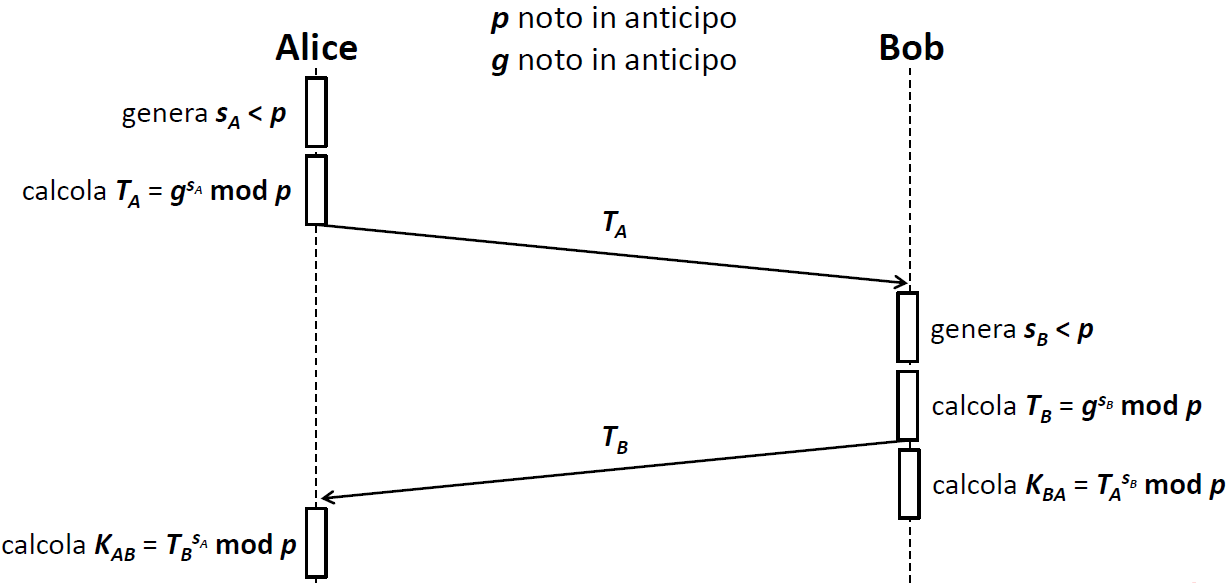
\includegraphics[scale=0.5, keepaspectratio]{Immagini/chiave_pubblica/DiffieHellman_schema.png}}
	\caption{Diffie-Hellman: schema}
	\end{figure}

Tuttavia, dati $p$, $g$, $T_{A}$ e $T_{B}$, è possibile calcolare $s_{A}$, $s_{B}$ oppure $g^{s_{A}s_{B}}$? Si può ottenere $s_{A}$ da $g^{s_{A}}$ tramite logaritmo discreto $dlog_{g} \, g^{s_{A}}$, ma al momento non sono note tecniche per calcolare tale quantità in un tempo ragionevole, anche conoscendo $g^{s_{A}}$ e $g^{s_{B}}$.

La vulnerabilità di Diffie-Hellman è che tale algoritmo non fornisce alcuna prova di autenticazione: Alice non può essere certa che $T_{B}$ sia stato inviato da Bob e non da un impostore; allo stesso modo, Bob non può essere certa che $T_{A}$ sia stato inviato da Alice e non da
un impostore. E' quindi possibile che un impostore, Mr. X, intercetti e modifichi i messaggi facendo credere a Bob di comunicare con Alice e
viceversa. Alice e Bob non hanno modo di rendersi conto dell'attacco in atto. Un attacco di questo tipo viene detto Man-in-the-Middle(o Bucket Brigade Attack): Alice pensa che $K_{AX}$ sia la chiave segreta $K_{AB}$ che condivide con Bob; Bob pensa che $K_{bX}$ sia la chiave segreta $K_{BA}$ che condivide con Alice; invece, Mr. X ha due chiavi segrete: \begin{itemize}
\item $K_{XA}$ per comunicare con Alice;
\item $K_{XB}$ per comunicare con Bob.
\end{itemize}
Questo perchè Mr. X conosce $g$ e $p$, quindi si calcola $s_{x}<p$ e $T_{x}=g^{s_{x}} \, mod \, p$ e li invia sia ad Alice che a Bob. Tale attacco è un attacco all'integrità. 
\begin{figure}[htbp]
	\centering%
	\subfigure%
	{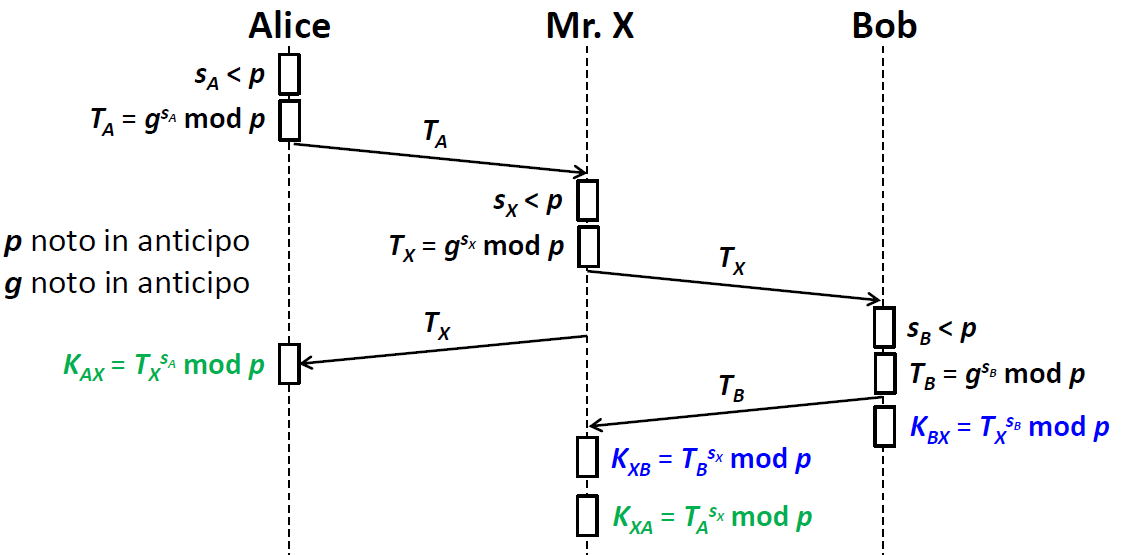
\includegraphics[scale=0.5, keepaspectratio]{Immagini/chiave_pubblica/DiffieHellman_maninthemiddle.png}}
	\caption{Man-in-the-Middle Attack}
	\end{figure}
	
Come risolvere tale problema? 
\begin{itemize}
\item \textbf{Autenticazione via password}: \\ Ipotesi: Alice e Bob si sono preliminarmente accordate su una coppia di password($pwd_{A}$, password che Alice invia a Bob; $pwd_{B}$, password che Bob invia ad Alice). Si consideri allora la seguente procedura di autenticazione, dove $K_{AB}$ è la chiave segreta condivisa ottenuta con Diffie-Hellman: \begin{enumerate}
\item scambio chiavi Diffie-Hellman;
\item Alice invia un messaggio cifrato con $K_{AB}$ e $pwd_{A}$;
\item Bob invia un messaggio cifrato con $K_{BA}$ e $pwd_{B}$.
\end{enumerate}
Il problema è che l'autenticazione via password, se è in corso un attacco Man-in-the-Middle, non funziona: Mr. X può decifrare tutte i messaggi che riceve da Alice con $K_{AX}$, cifrarli con $K_{XB}$ e inviarli a Bob. Viceversa, può decifrare tutte i messaggi che riceve da Bob con $K_{XB}$, cifrarli con $K_{AX}$ e inviarli ad Alice.
\begin{figure}[htbp]
	\centering%
	\subfigure%
	{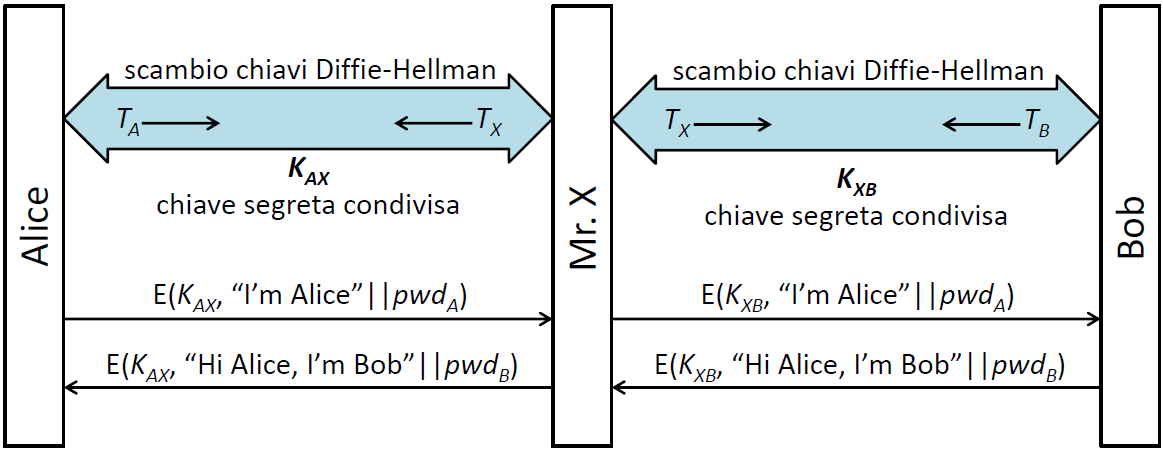
\includegraphics[scale=0.5, keepaspectratio]{Immagini/chiave_pubblica/DiffieHellman_passauth.png}}
	\caption{Autenticazione via password}
	\end{figure}
\item Anche altri tipi di proposte sono insufficienti(timestamp, domande personali..). Il problema è che Diffie-Hellman effettua delle operazioni invertibili(cifratura/decifratura) ed è sicuro solo nel caso di attacchi passivi(un intruso intercetta i messaggi, ma non li modifica). E' necessario proteggere l'integrità, per cui si adottano due strategie generali: Diffie-Hellman con Numeri Pubblici e Scambio Diffie-Hellman Autenticato.	
\end{itemize}

\textbf{Diffie-Hellman con Numeri Pubblici}. Un possibile modo per sventare attacchi attivi è evitare che $p$, $g$, $s_{A}$, $s_{B}$, $T_{A}$ e $T_{B}$ vengano generati/calcolati ad ogni scambio. $p$, $g$, $T_{A}$ e $T_{B}$ potrebbero essere resi pubblici in una repository fidata, con $p$ e $g$ uguali per tutti gli utenti, mentre ogni utente U pubblica il proprio valore $T_{U}$, mantenendo privato il segreto $s_{U}$. Ne consegue che, se un avversario non è in grado di accedere alla repository e di modificare i valori pubblici, allora Diffie-Hellman diventa sicuro anche nel caso di attacchi attivi. Inoltre, non è più necessario lo scambio dei valori $T_{A}$ e $T_{B}$: consultando la repository ogni utente A può ottenere la chiave $K_{AB}$ che condividerebbe con l'utente B. \\

\textbf{Scambio Diffie-Hellman Autenticato}. Alice e Bob conoscono un qualche tipo di informazione che permette loro di autenticarsi reciprocamente, ovvero una chiave segreta condivisa $K^{AB}$, da non confondere con la chiave concordata con Diffie-Hellman $K_{AB}$, la propria coppia <chiave privata, chiave pubblica> e la chiave
pubblica dell'altro. Si possono usare tale(i) informazione(i) per provare che sono realmente loro, e non un impostore, coloro che generano i valori di Diffie-Hellman $g$, $p$, $T_{A}$ e $T_{B}$. Tale prova può avvenire sia contestualmente che dopo lo scambio Diffie-Hellman esaminato in precedenza. 

Notazione adottata: \begin{itemize}
\item $K^{AB}$: chiave segreta condivisa tra Alice e Bob prima di effettuare lo scambio Diffie-Hellman.
\item $K_{AB}$: chiave concordata con Diffie-Hellman.
\item $K^{AB}$ \{msg\} : cifratura di msg con la chiave segreta $K^{AB}$, cioè $E(K^{AB}, msg)$.
\item $\{msg\}_{Bob}$ : cifratura di msg con la chiave pubblica di Bob, cioè $E(PU_{Bob}, msg)$.
\item $[msg]_{Bob}$ : firma di msg con la chiave privata di Bob, cioè
$E(PR_{Bob}, msg)$.
\end{itemize}
Di seguito sono indicate alcune possibili soluzioni per lo scambio Diffie-Hellman autenticato:
\begin{itemize}
\item Autenticazione contestuale allo scambio Diffie-Hellman: \begin{enumerate}
\item Cifrare lo scambio Diffie-Hellman con la chiave segreta $K^{AB}$.
\begin{figure}[htbp]
	\centering%
	\subfigure%
	{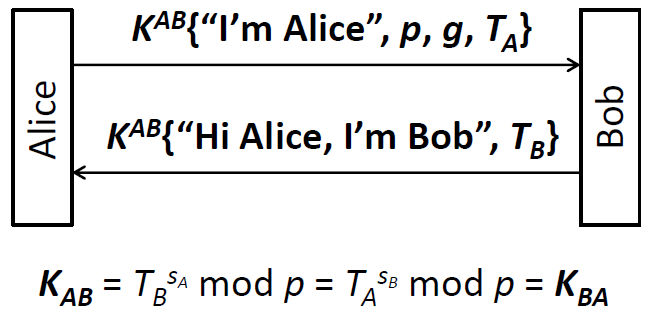
\includegraphics[scale=0.5, keepaspectratio]{Immagini/chiave_pubblica/DiffieHellman_auth1.png}}
	\caption{Utilizzo $K^{AB}$.}
	\end{figure}
\item Cifrare il valore Diffie-Hellman con la chiave pubblica dell'altro interlocutore(figura \ref{fig:auth2}).
\begin{figure}[htbp]
	\centering%
	\subfigure%
	{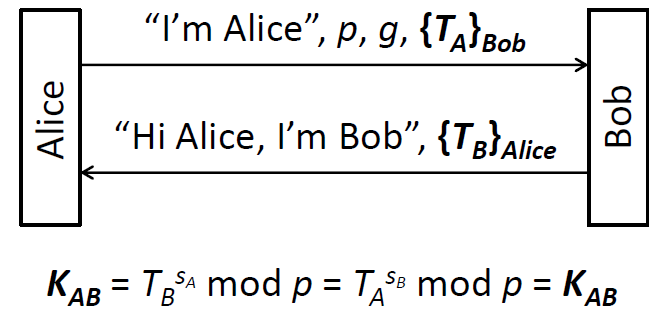
\includegraphics[scale=0.5, keepaspectratio]{Immagini/chiave_pubblica/DiffieHellman_auth2.png}}
	\caption{Utilizzo chiave pubblica dell'altro interlocutore.}
	\label{fig:auth2}
	\end{figure}
\item Firmare il valore Diffie-Hellman con la propria chiave privata(figura \ref{fig:auth3}).
\begin{figure}[htbp]
	\centering
	\subfigure
	{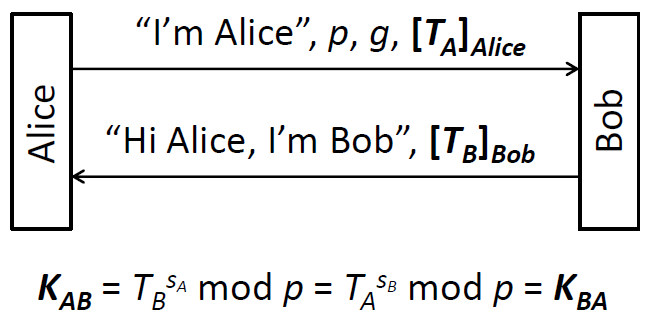
\includegraphics[scale=0.5, keepaspectratio]{Immagini/chiave_pubblica/DiffieHellman_auth3.png}}
	\caption{Utilizzo propria chiave privata.}
	\label{fig:auth3}
	\end{figure}
\end{enumerate}
\item Autenticazione successiva allo scambio Diffie-Hellman(figura \ref{fig:auth45}):
\begin{enumerate}
\item Dopo lo scambio Diffie-Hellman, trasmettere un hash della chiave concordata $K_{AB}$, del proprio nome e della chiave segreta $K^{AB}$.
\item Dopo lo scambio Diffie-Hellman, trasmettere un hash del valore
Diffie-Hellman trasmesso e della chiave segreta $K^{AB}$.
\end{enumerate}
\end{itemize}
\begin{figure}[htbp]
	\centering
	\subfigure
	{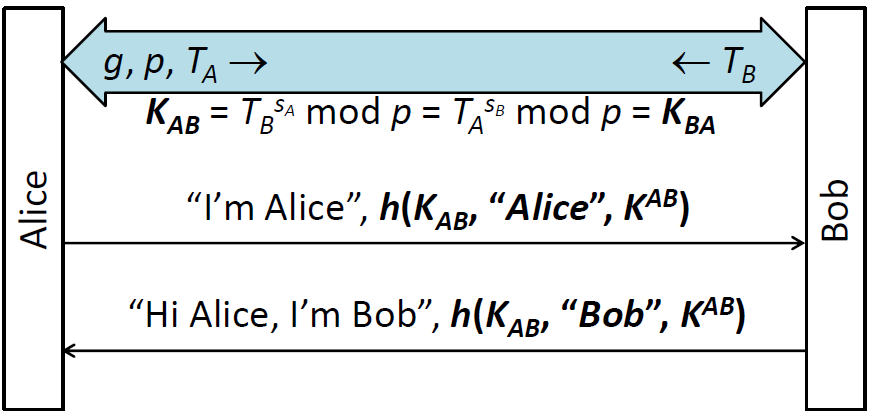
\includegraphics[scale=0.5, keepaspectratio]{Immagini/chiave_pubblica/DiffieHellman_auth4.png}}
	\hspace{2mm}
	\subfigure
	{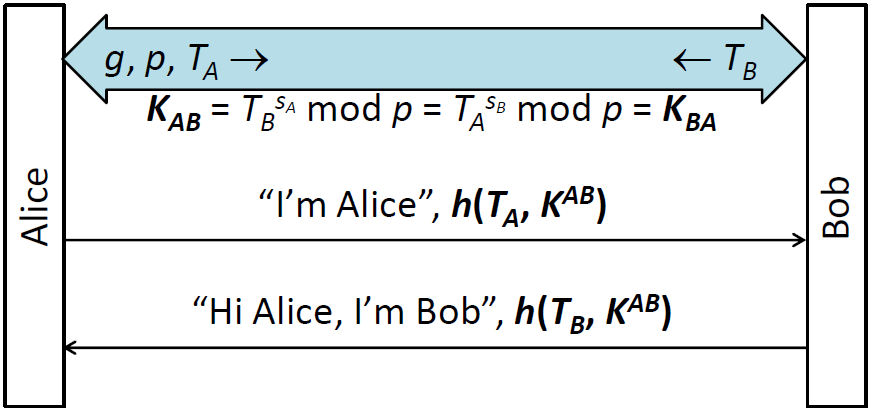
\includegraphics[scale=0.5, keepaspectratio]{Immagini/chiave_pubblica/DiffieHellman_auth5.png}}
	\caption{Autenticazione successiva allo scambio Diffie-Hellman.}
	\label{fig:auth45}
	\end{figure}

Oltre alla mancanza di autenticazione, Diffie-Hellman classico presenta anche lo svantaggio che, la comunicazione cifrata con la chiave concordata, può avvenire soltanto dopo l'esecuzione di uno scambio attivo. In pratica, Alice non può inviare un messaggio cifrato a Bob prima di ricevere $T_{B}$. Tale problema puo essere ovviato
introducendo le chiavi pubbliche Diffie-Hellman: una chiave pubblica D-H è una tripla $<p, g, T>$, dove $T = g^s \, mod \, p$, dove $s$ è la corrispondente chiave privata. Le chiavi pubbliche vanno custodite in un luogo fidato e accessibile da tutti in modo sicuro. La chiave pubblica di Bob è $<p_{B}, g_{B}, T_{B}>$. \\

Di seguito(figura \ref{fig:authex}), mostriamo un esempio di procedura che consenta ad Alice di inviare un messaggio cifrato a Bob, con la chiave concordata $K_{AB}$, anche se Bob risulta essere inattivo, cioè Alice deve essere in grado di cifrare senza dover attendere alcuna risposta da Bob, il quale, una volta attivo, dovrà poter calcolare $K_{AB}$ e decifrare il messaggio:
\begin{enumerate}
\item Alice genera $s_{A}<p_{B}$, calcola $T_{A}^{*}=g_{B}^{s_{A}} \, mod \, p_{B}$ e $K_{AB}=T_{B}^{S_{A}} \, mod \, p_{B}$.
\item Poi cifra il messaggio $msg=E(K_{AB},msg)$ e lo invia a Bob assieme a $T_{A}^{*}$.
\item Bob, una volta attivo, calcola  $K_{BA}=(T_{A}^*)^{S_{B}} \, mod \, p_{B}$.
\item Decifra $E(K_{AB},msg)$, ottenendo $msg=D(K_{BA},E(K_{AB},msg))$.
\end{enumerate}
\begin{figure}[htbp]
	\centering%
	\subfigure%
	{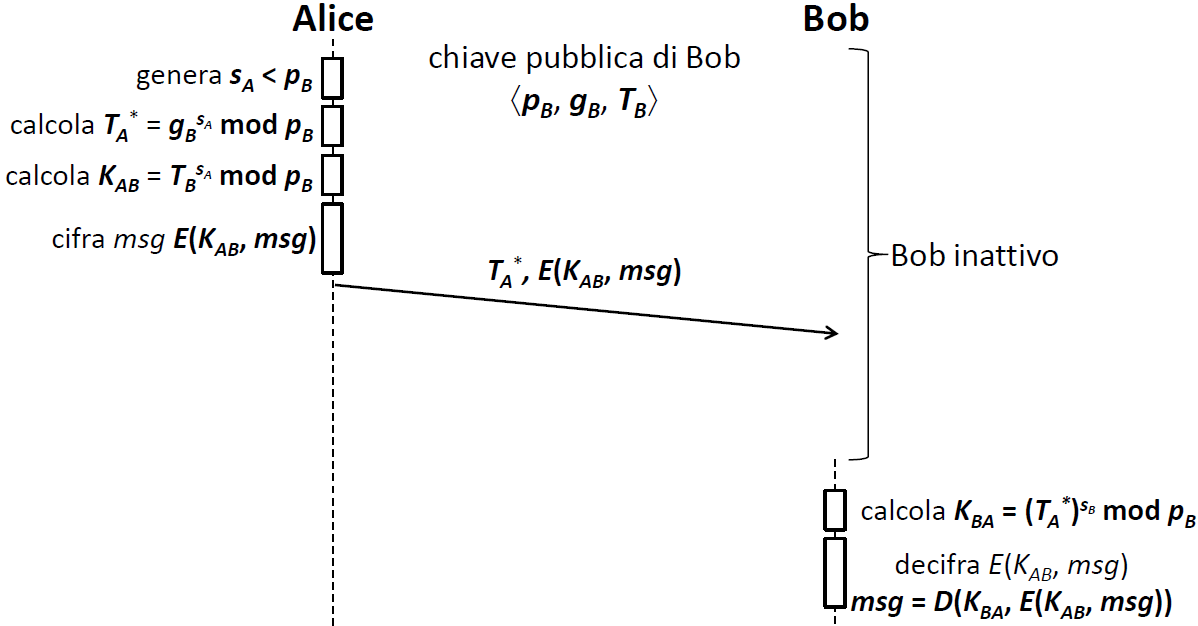
\includegraphics[scale=0.6, keepaspectratio]{Immagini/chiave_pubblica/DiffieHellman_pubseckey.png}}
	\caption{Chiavi pubbliche/private Diffie-Hellman}
	\label{fig:authex}
\end{figure} 

\section{Zero Knowledge Proof System}

La dimostrazione della conoscenza di un segreto è alla base di molte tecniche di autenticazione. Nelle tecniche di autenticazione a chiave segreta, il segreto è appunto la chiave condivisa tra i due principal. Nei protocolli a chiave pubblica il segreto è noto solo ad un principal, il quale deve dimostrare all'altro che detiene il segreto senza fornire delle informazioni che possano consentire ad un impostore di eseguire la prova. \\
Una dimostrazione quindi è a \textit{conoscenza zero}(\textbf{Zero Knowledge Proof, ZKP}) se permette di provare la conoscenza di un segreto, che deve essere associato alla chiave pubblica, senza fornire delle informazioni che permettano ad un impostore di eseguire la prova: \begin{itemize}
\item la prova non deve rivelare il segreto;
\item la prova non deve rivelare eventuali informazioni, che pur non essendo il segreto, consentano comunque ad un impostore di effettuare la prova.
\end{itemize}
Le dimostrazioni a conoscenza zero sono impiegate nei protocolli/sistemi di autenticazione(detti \textbf{Zero Knowledge Proof Systems, ZKPS}). RSA è un esempio di ZKPS: è possibile provare la conoscenza di un segreto associato alla chiave pubblica(si pensi alla firma di una sfida), senza rivelare la chiave privata o altre informazioni che
permettano ad un impostore di impersonare il proprietario
della chiave privata. Tuttavia, esistono ZKPS molto più efficienti di RSA, anche se non permettono di cifrare e/o di firmare. \\

Uno schema di autenticazione a conoscenza zero(\textbf{Zero Knowledge Authenication Scheme, ZKAS}) consiste in un'autenticazione che sfrutta una \textit{ZKP}. Non si tratta di una tecnica deterministica, ma
probabilistica(anche RSA in fondo è probabilistica). Deve poter essere resa arbitrariamente piccola la probabilità che un dimostratore onesto fornisca una prova errata; un verificatore onesto fornisca una verifica errata quando il dimostratore è onesto; un dimostratore disonesto fornisca una prova corretta. 

Uno schema di autenticazione a conoscenza zero deve soddisfare i seguenti requisiti: \begin{itemize}
\item[a.] ad ogni entità è associato un segreto privato $s$ e
una chiave pubblica $k_{s}$, cioè una coppia $<s, k_{s}>$. Ovviamente, $k_{s}$ non deve esporre $s$;
\item[b.] l'autenticazione consiste nel provare la conoscenza del segreto $s$;
\item[c.] la prova deve essere a conoscenza zero, cioè le informazioni addotte dal dimostratore non devono poter essere riutilizzate con successo(in seguito) da un impostore, quindi la prova non consente di rivelare $s$;
\item[d.] chi non conosce il segreto $s$ non deve poter eseguire la prova con successo;
\item[e.] chi non conosce il segreto $s$ deve poter verificare la correttezza della prova utilizzando la chiave pubblica $k_{s}$ dell'entità che si sta autenticando(senza la chiave pubblica non deve essere possibile verificare la correttezza della prova).
\end{itemize}

\subsection{ZKAS basato su MSR}

Di seguito mostriamo un protocollo di autenticazione, estremamente efficiente, che sfrutta un problema difficile nell'ambito dell'aritmetica modulare. A rigore tale schema di autenticazione non è
completamente a conoscenza zero, anche se nella pratica può considerarsi tale. \\
Il problema che viene sfruttato è il problema della radice quadrata modulare(\textbf{Modular Square Root, MSR}): dati un numero intero semiprimo grande $n=pq$, con $p$ e $q$ numeri primi grandi, $m<n$ intero assegnato(avente una radice quadrata ordinaria non intera), trovare un numero intero $s$ tale che $s^2 \, mod \, n=m$ è un problema difficile almeno quanto fattorizzare un numero intero.
Dunque, tale protocollo consiste dei seguenti passi: \begin{enumerate}
\item \textbf{Generazione delle chiavi}. Peggy(il dimostratore) calcola la chiave pubblica $<n,v>$, dove $n=pq$ come in RSA, $v$ è un numero di cui Peggy conosce la radice quadrata modulare(ottenere $v$ è semplice, basta scegliere un numero random $s$ e porre $v = s^2 \, mod \, n$; $s$ è la chiave privata di Peggy da non rivelare; $<n,v>$ va divulgata a tutto il mondo.
\item \textbf{Autenticazione}. \begin{itemize}
\item Peggy sceglie $k$ numeri random $r_{1},r_{2},..,r_{k}$;
\item Per ogni $r_{i}$ invia a Victor $r_{i}^2 \, mod \, n$;
\item Victor attribuisce a ciascun $r_{i}^2$ che vale 0 o 1 e la comunica a Peggy;
\item Peggy invia a Victor $sr_{i} \, mod \, n$ per ciascun $r_{i}^2$ etichettato con 1 e $r_{i} \, mod \, n$ per ciascun $r_{i}^2$ etichettato con 0;
\item Victor eleva al quadrato ciascun numero della risposta di Peggy e verifica che tale quadrato valga $vr_{i}^2 \, mod \, n$ se il corrispondente $r_{i}^2$ aveva etichetta 1, oppure $r_{i}^2 \, mod \, n$ se il corrispondente $r_{i}^2$ aveva etichetta 0.
\end{itemize}
\end{enumerate}
\begin{figure}[htbp]
	\centering%
	\subfigure%
	{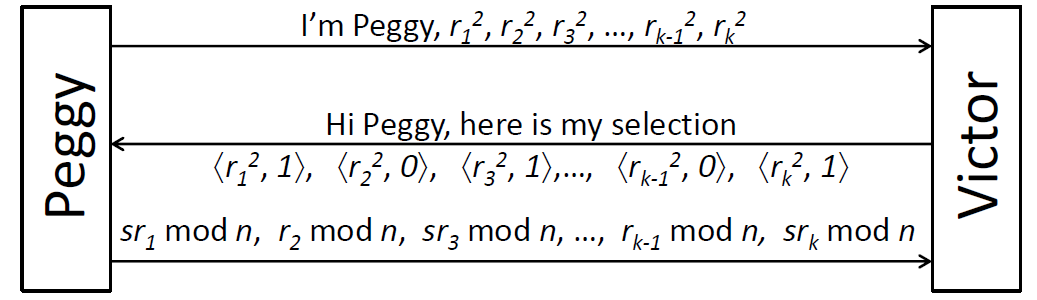
\includegraphics[scale=0.6, keepaspectratio]{Immagini/chiave_pubblica/zkasmsr_auth.png}}
	\caption{}
\end{figure}

Supponiamo che Fred voglia impersonare Peggy. Allora egli è in grado di rispondere in modo corretto agli $r_{i}^2$ che Victor etichetta con 0(Fred può scegliere a suo piacimento gli $r_{i}$), ma non è in grado di rispondere agli $r_{i}^2$ etichettati con 1. In assenza di etichette 0, infatti, il protocollo si semplificherebbe: Peggy si limiterebbe ad inviare delle coppie $<r_{i}^2, sr_{i} \, mod \, n>$, tuttavia non si avrebbe più un protocollo a conoscenza zero, poichè Fred potrebbe usare una precedente sequenza inviata di Peggy ed impersonarla con successo. Invece, l'etichettatura scelta in modo casuale da Victor implica che Fred ha una probabilità del 50\% di
rispondere in modo corretto ad ogni $r_{i}^2$. Fred potrebbe generarsi autonomamente gli $r_{i}$, ma in tal caso non saprebbe rispondere agli $r_{i}^2$ con etichetta 1 oppure potrebbe usare un insieme di $r_{i}^2$ etichettati in passato con 1 in una precedente autenticazione, ma allora non conoscerebbe i corrispondenti $r_{i}$ e non saprebbe rispondere nel caso in cui l'etichetta è 0. Se $k$ è sufficientemente grande la probabilità che Fred impersoni correttamente Peggy tende a 0. \\
ZKAS basato su MSR è molto più efficiente di RSA. Infatti, assumendo $k = 30$, Peggy deve effettuare 45 operazioni modulari(30
quadrati più una media di 15 moltiplicazioni per $s$) e Victor deve effettuare lo stesso numero di operazioni di Peggy; usando RSA Peggy deve eseguire una esponenziazione modulare che consiste in una media di 768 moltiplicazioni modulari mentre Victor se la cava con 3 moltiplicazioni nel caso in cui $e = 3$.
